\section{Clustering comparison}
	
	In this section a series of clustering algorithm are compared.
	

	\subsection{Purpose}
	
		The purpose of this project is to check the performance of different clustering algorithms when applied to our different datasets.\\
		
		To do this, we create ground truth clusters of zernike mode coefficients (for example for 2 zernike modes we define two value ranges of [-1, -0.8] and [0.8, 1] which will create 4 different clear clusters) and from them we create the PSFs, LP coefficients and PL output fluxes.\\
		
		We evaluate the following clustering algorithms:
		\begin{itemize}
			\item K-Means
			\item DBSCAN
			\item HDBSCAN
			\item Agglomerative
		\end{itemize}
	

	\subsection{The data}
	
		There are 4 different types of datasets:
		\begin{itemize}
			\item Zernike coefficients
			\item PSF
			\item LP coefficients
			\item Photonic Lantern Output fluxes
		\end{itemize}
		
		The paths to the datasets can be found in the file \href{https://github.com/Dacarpe03/PLImageReconstruction/blob/main/Utils/minidataset_constants.py}{minidataset\_constants.py}.\\
		
		We have used 2, 5, 9 and 14 zernike modes to create 4 datasets of 5000 datapoints each.
		

	\subsection{Results}
	
		\begin{figure*}[ht!]
			\centering
			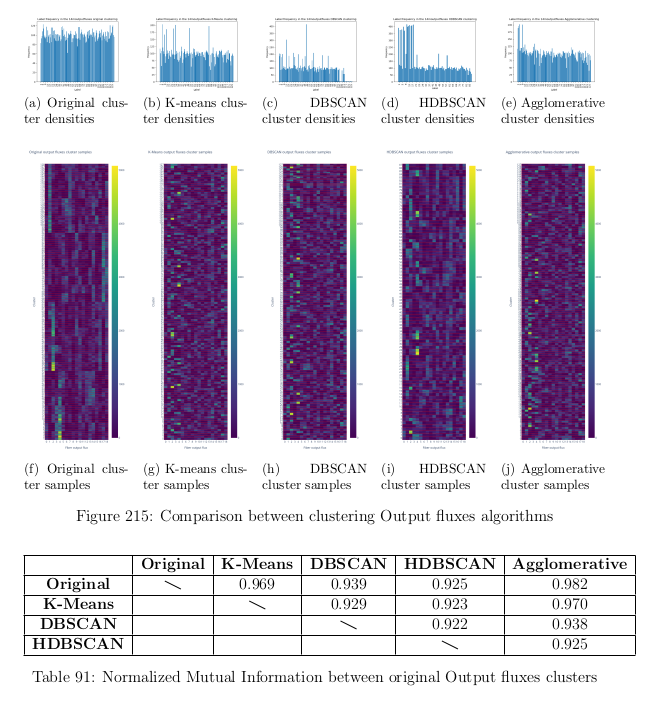
\includegraphics[width=0.9\textwidth]{
		draft-20clustersummary.png}
			\caption{Summary of clustering 20 zernike modes dataset}
		\end{figure*}
		\FloatBarrier
		
		The best clustering algorithm is the Agglomerative followed by K-Means, although K-Means takes a lot of time.
	
	
	\subsection{Code}

		\begin{itemize}
			\item The code to generate the datasets can be found in the notebook \href{https://github.com/Dacarpe03/PLImageReconstruction/blob/main/PSFReconstruction/DataNotebooks/MinidatasetZernikePSFGeneration.ipynb}{MinidatasetZernikePSFGeneration.ipynb}
			\item The code to process the datasest can be found in the notebook \href{https://github.com/Dacarpe03/PLImageReconstruction/blob/main/PSFReconstruction/DataNotebooks/MinidatasetProcessing.ipynb}{MinidatasetProcessing.ipynb}
			\item The code to reduce dimensionality of the data with UMAPs and PCAs can be found in the notebook \href{https://github.com/Dacarpe03/PLImageReconstruction/blob/main/PSFReconstruction/DataNotebooks/MinidatasetDimensionalityReduction.ipynb}{MinidatasetDimensionalityReduction.ipynb}
			\item The code to cluster the minidatasets is divided in a notebook per set of zernike modes, for example to see the clustering for the 14 zernike mode related datasets see notebook \href{https://github.com/Dacarpe03/PLImageReconstruction/blob/main/PSFReconstruction/DataNotebooks/Minidataset14modesClustering.ipynb}{Minidataset14modesClustering.ipynb}
		\end{itemize}
		
		
	\subsection{Detailed results}
	
		For a detailed report on the datasets, results and plots see Part IV to VII from \filename{appendix.pdf}.